\chapter{Dataset}
\label{ch:dataset}
%poichè non erano presnti dataset adui suabili, ce ne siamo fatti uno noi. Poi per ogni metodo verranno esplicitati i dati usati.

The importance of using public data sets for algorithm evaluation is very important. Only in this way can a direct comparison be made between the different approaches to determine which of these is actually the best. There are publicly available datasets for the fall detection task, the majority of them are all related to wearable or vision sensors and often include both types \cite{spinsantefalldata, kwolek2014human, charfi2013optimized, s140610691, s17071513}. Since in this work, we face the problem fall detection from an audio perspective, only one dataset containing audio recording has been found \cite{cirdodataset}. However, the audio files available in the dataset are suitable for speech recognition related works rather than sound event detection. In fact, only the utterance of short sentences or interjections of the actors involved during the human falls recordings have been annotated. As in this work, several data-driven approaches for pattern recognition produced by the sound generated by the human fall are presented, the dataset \cite{cirdodataset} result useless. Given the lack of available audio data sets, we have created a suitable audio dataset in order to assess the proposed approaches. This choice was also forced by the fact that in these works an innovative acoustic sensor was explicitly developed for the fall detection and described in \secref{sec:sensor} has been used.
In this chapter, the instrumentation, the procedure for recording the audio corpus and its composition are described.

\section{The floor acoustic sensor}
\label{sec:sensor}

\begin{figure}[t]
	\centering
	\includegraphics[width=0.8\textwidth]{img/AcousticSensor.pdf}
	\caption{The floor acoustic sensor: conceptual scheme. \mbox{1 - The} outer container. \mbox{2 - The} inner container. \mbox{3 - The} microphone slot. \mbox{4 - The} membrane touching the floor.}
	\label{fig:case}
\end{figure}
The floor acoustic sensor (FAS) is composed of a resonant enclosure and a microphone located inside it (\figref{fig:case}) \cite{Olivetti15}. At the bottom of  the enclosure, a membrane  is in direct contact with the floor and guarantees the acoustic coupling with the surface. The inner container accommodates the microphone and is where the acoustic resonance phenomenon takes place. It can be covered by a layer of acoustic isolation material and it is enclosed by the outer container that further reduces the intensity of the acoustic waves that propagate through air. The enclosure has been manufactured in Polylactic Acid with a 3D printer, its diameter is 16.5\,cm and its height 5.5\,cm.

%The acoustic sensor used in the sound database acquisition (as described in \secref{Experiments}) is depicted in \figref{fig:meringa}. The dimensions of the acoustic sensor are the following: 16.5\,cm of diameter and 5.5\,cm of height. The material used for the sensor case, developed through the 3D printing technology, is Polylactic Acid. %No acoustic isolation material has been inserted into the space between the inner and outer container.

Regarding the microphone, an AKG C 400 BL\footnote{http://www.akg.com/pro/p/c400-bl} has been inserted in the enclosure. The outer case of the microphone has been removed to extract the capsule that has then been inserted in the sensor enclosure. The AKG C 400 BL is characterized by an hypercardiod directivity pattern, thus it has been oriented so that the maximum gain is towards floor.

\begin{figure}[t]
	\centering
	\includegraphics[width=0.8\columnwidth]{img/FAS_front_little.jpg}
	\caption{A picture of the floor acoustic sensor used during the recordings.} \label{fig:meringa}
\end{figure}

\section{The fall events dataset: A3Fall}
\label{sec:dataset}
The performance of the floor acoustic sensor has been evaluated on a corpus of audio events corresponding to falls of several objects recorded in different conditions\footnote{The dataset is available at the following URL: \url{http://www.a3lab.dii.univpm.it/research/fasdataset}}. The dataset has been specifically created by the authors and it will be presented in this section.

\subsection{The recording setup}
Fall events have been recorded in 3 different rooms with the following characteristics:
\begin{itemize}
	\item The first, is a rectangular room, hereafter named R0, measuring about 7\,m\,$\times$\,2\,m (\figref{fig:room}). The room is particularly suitable for the propagation of acoustic waves through the floor since it is obtained from a cantilever beam. In addition, the considerable distance of the supporting pillars facilitates the transmission of a fall vibrations through the floor.
	\item the second location for the recording was the university auditorium room (R1) in which the flooring is composed of fitted carpet. This makes it particularly suitable for evaluating system performance on surfaces with acoustical behavior that can mitigate the impact sound transmitted through the floor and in the air; all the recordings were performed near the auditorium stage in an area of 8$\times$3\,m.
	\item a recording studio (R2) was selected as the third location for its particular characteristics. Here, it was possible to make the acquisitions by placing the sensors in the live room while the audio events were performed in the control room. In particular, the sensors were positioned immediately behind the soundproof wall with the window overlooking the live room. The size of the live room is 5$\times$7\,m, while the size of the control room is 3$\times$8\,m.
\end{itemize}

  The recording equipment comprises the floor sensor, a linear array of three aerial microphones (the same AKG 400 BL included in the floor sensor) and a Presonus AudioBox 44VSL sound card connected to a laptop. The microphones of the array are separated by 4\,cm and positioned on a table 80\,cm high. Signals were sampled at 44.1\,kHz with a resolution of 32\,bits. Levels were calibrated to assure the maximum dynamic range at the smallest distance.

\subsection{Description}
In \tableref{tab:numDataset} the composition of the dataset is summarized.
For the R0, the dataset comprises recordings of fall events related to everyday objects and to a human mimicking doll. The objects were chosen according to the recent literature on the topic \cite{alwan2006smart} and are the following: a ball, a metal basket, a book, a metal fork, a plastic chair, and a bag (\figref{fig:objects}). Objects have been dropped at four distances from the sensors, i.e., 1\,m, 2\,m, 4\,m, and 6\,m, and with various angles in order to reproduce realistically different fall patterns. With the exception of the chair and the basket, which have been overturned from their natural position, half of the falls has been performed at a height of 0.5\,m and the other half at 1\,m. For each object and for each distance, 16 fall events have been performed for a total of 64 events per object. Instead, the chair has been overturned 8 times for each side of fall (back, front, side) and for each distance, thus obtaining a total of 96 events.

\begin{table}[t]
	\caption{Composition of the A3Fall-v2.0 dataset.}
	\label{tab:numDataset}
	\begin{center}
		\begin{tabular}[t]{c|ccc}
			
			\hline
			\textbf{Class} & \textbf{R0} & \textbf{R1} & \textbf{R2} \\ %\cline{2-5} 
			%& \hspace{8pt}Clean\hspace{8pt}  & \hspace{6pt}Clean\hspace{6pt}   \\ 
			\hline
			&\multicolumn{3}{c}{Nr. of occurrences}\\
			Basket      			& 64    &   40 	&   40    	\\
			Fork        			& 64    &   40 	&   40     	\\
			Ball       				& 64    &   40	&   40    	\\
			Book        			& 64    &   40	&   40    	\\
			Bag         			& 64    &   30 	&   40    	\\
			Chair       			& 96    &   40 	&   40    	\\
			Table       			& 0   	&   40 	&   40    	\\
			Guitar Slide       		& 0   	&   40 	&   40    	\\
			Nipper       			& 0    	&   40 	&   40    	\\
			Keys       				& 0    	&   40 	&   40    	\\
			Hook       				& 0    	&   40 	&   40    	\\
			Coat Hook       		& 0    	&   40 	&   40    	\\
			$\,$ Manikin Doll $\,$ 	& 44    &   0 	&   0    	\\
			$\,$ Human Fall $\,$ 	& 0    	&   40 	&   40    	\\
			\hline
			&\multicolumn{3}{c}{Total length (s)}\\			
			%			Human Activity  		& 1135  &   3050&   580   	\\
			%			Music					& 1395  &	4330&   3345  	\\
			%			Television				& 0   	&	1675&   1625  	\\
			Background  			& 2530  &   9055&   5550   	\\
			\hline
		\end{tabular}
	\end{center}
\end{table}

\begin{figure}[t]
	\centering
	\includegraphics[width=0.4\textwidth]{img/oggetti_cadute3.jpeg}
	\caption{Objects employed for creating the fall events dataset.}\label{fig:objects}
\end{figure}

Human falls have been simulated by employing the ``Rescue Randy'' doll\footnote{http://www.simulaids.com/1475.htm}, a professional equipment employed in water rescues. It weights 75\,kg, it is 1.85\,m high, and it is equipped with articulated joints. The doll is made of vinyl and its weight is distributed according to the human weight distribution chart. The doll has been dropped from upright position and from a chair, both forward and backward, for a total of 44 events (\figref{fig:randy}). Differently from the everyday objects, the distribution of the fall events with the distance is not uniform: 10 events have been performed from 2\,m, 18 from 4\,m (7 of which from the chair), and 16 from 6\,m (6 of which from the chair).

Moreover, several backgrounds sounds has been added to the dataset. 
Normal activities sounds have been recorded while persons were performing common actions, such as walking, talking, and dragging chairs. Three musical tracks have been played from a loudspeaker and acquired back with the FAS. The first track contained classical music\footnote{W. A. Mozart, ``Piano trio in C major''}, while the second\footnote{Led Zeppelin, ``Dazed and confused''} and the third\footnote{Led Zeppelin, ``When the levee breaks''} rock music. Musical tracks and normal activities sounds have been divided in segments whose lengths have mean and standard deviation estimated from instances of fall events. In addition, they have been employed alone and to create noisy versions of human and object falls occurrences in order to assess the algorithm in presence of interferences. 

In R2 and R1 other every-days objects,in addition to those used in R0, have been recorded for a total of 12 different object fall classes and 1420 instances. While the manikin doll has been used only in R0, in R1 and R2 a total 80 human falls have been performed by 4 people. These falls were performed in different ways: forward, backward and on the side, trying to use the arms to cushion the fall and without any protections. As in R0, also in R2 and R2 all events were performed from 1, 2, 4 and 6 m away from the FAS.

\begin{figure}[t]
	\centering
	\begin{subfigure}[b]{0.40\textwidth}
		\includegraphics[width=\textwidth]{img/impalcatura.jpg}
		\caption{Fall from upright position.}\label{fig:randy_upright}
	\end{subfigure}
	\begin{subfigure}[b]{0.40\textwidth}
		\includegraphics[width=\textwidth]{img/rndy_caduta_sedia.jpg}
		\caption{Fall from the chair.}\label{fig:randy_chair}
	\end{subfigure}
	\caption{Falls of the ``Rescue Randy'' doll from upright position (a) and from the chair (b).}\label{fig:randy}
\end{figure}

\begin{figure}[t]
	\centering
	\includegraphics[width=\columnwidth]{img/room_experiments.pdf}
	\caption{The recording room: the letters A, B, C and D indicate the positions of fall events.}
	\label{fig:room}
\end{figure}

As shown in \tableref{tab:numDataset} background noises have been recorded also in R1 and R2 rooms rooms, which include: human activities noise as, i.e., footsteps, human and phone conversation, dragging objects and so on; classic, rock and pop music played from loudspeakers; TV shows like newscast and satiric.

Since the data relating to rooms R1 and R2 have been collected at different times to those of room R0, in the following chapters, for each proposed approach, it will be specified which subset of the total dataset has been used as well as the usage of the noisy version of falls events.


\subsection{Signal analysis}\label{ssec:sig_analysis}
The signal related to the same fall event acquired with the floor sensor and with the aerial microphone exhibits different spectral characteristics. In this section and in depth analysis of the audio signals acquired in the R0 room is presented. \figref{fig:spectrograms} shows the spectrograms of a doll fall acquired with the floor sensor (above) and with the aerial microphone (below) in the clean acoustic condition. Observing the figures, it can be noticed that the aerial microphone is more sensitive to high frequencies, in particular to the ones above 1.5\,kHz. On the contrary, the majority of the energy of the signal acquired with the floor sensor concentrates below 1\,kHz. 

This is even more evident by plotting the values of the mel coefficients (\figref{fig:mel}): the first and second mel channels of the FAS, corresponding to the frequency bands 0--128.10\,Hz and 61.30-200.60\,Hz, are higher respect to the aerial microphone. Channels 3 to 7, respectively corresponding to bands 128.10--279.50\,Hz and 458.70--670.70\,Hz, are almost equivalent, while from channel 8 (560.30--790.80\,Hz) to 29 (6654.60--8000.00\,kHz) the aerial microphone mels are greater.

\begin{figure}[t]
	\centering
	\begin{subfigure}[b]{0.8\textwidth}
		\includegraphics[width=\textwidth]{img/spettro_fas}
		\caption{Spectrogram of the signal acquired with the floor sensor.}
		\label{fig:spec_fas}
	\end{subfigure}
	\begin{subfigure}[b]{0.8\textwidth}
		\includegraphics[width=\textwidth]{img/spettro_mic}
		\caption{Spectrogram of the signal acquired with the aerial microphone.}
		\label{fig:spec_aer}
	\end{subfigure}
	
	\caption{Frequency content of the same fall event (file ``rndy\_d2st\_bar\_0.wav'') acquired with the FAS (a) and with the aerial microphone (b).}\label{fig:spectrograms}
\end{figure}

\begin{figure}[t]
	\centering
	\includegraphics[width=0.75\textwidth]{img/mel_dB}
	\caption{Average value of the mel channels.} \label{fig:mel}
\end{figure}

\begin{figure}[t]
	\centering
	\includegraphics[width=0.75\textwidth]{img/SNR_mel_channel}
	\caption{Average value of the SNR for each mel channel.} \label{fig:noisymel}
\end{figure}

The analysis of noisy signals highlights the different behaviour of the floor sensor respect to the aerial microphone in presence of external interferences. 
In fact, taking into account the backgrounds tracks as interferences, the floor sensor has a global signal-to-noise ratio (SNR) equal to 20.94\,dB and a segmental SNR equal to 7.28\,dB. The global SNR of the central aerial microphone is 8.92\,dB and the segmental SNR is -1.47\,dB. The values of the aerial microphone SNRs are thus considerably lower than the ones of the floor sensor.%: this highlights the superiority of the FAS respect to the aerial microphone in reducing sounds propagating through the air and not related to fall events.
The global SNR of the floor sensor noisy dataset is 13.66\,dB higher than the one of the aerial microphone, highlighting the superior ability of the former to isolate fall signals from external interferences. However, it is worth investigating how the SNR distributes over the frequency range of the acquired signals in order to have a better insight of the physical phenomenon. \figref{fig:noisymel} shows the SNR calculated for each mel channel and averaged across the noisy datasets. It can be noticed that the SNR of the floor sensor exceeds the one of the aerial microphone for channels below the fourth. Then, the opposite occurs and the SNR of the aerial microphone assumes greater values. The ``valley'' in the curves are due to the pitch of the music signal.


